{$\space$\par}
\vspace{0.5cm}
\justifying
\section*{{\bfseries \LARGE Questão 2 -} {\bfseries \large A figura abaixo representa medições de rádio feitas pelo radiotelescópio Big Ear em 1977. As observações destacadas pelo círculo vermelho onde se lê 6EQUJ5 ficaram conhecidas como Sinal Uau (ou Wow, como quiser). As letras e números representam uma escala de intensidade, segundo a ordem: 123456789ABCDEFGHIJKLMNOPQRSTU. A cada 2 segundos, a intensidade do sinal medido seria representada por uma dessas letras. Suponha que essa escala seja linear, tal que 1 represente intensidade 1, 7 represente intensidade 7, A represente intensidade 10, e assim por diante, até a letra U, que representa a intensidade 30. Cada coluna composta por um caracter representa uma série de medidas. Com base nos dados dessa figura, estime a probabilidade
do Sinal Uau ter sido um evento
aleatório.}}

\vspace{0.2cm}

\begin{figure}[h]
    \centering
    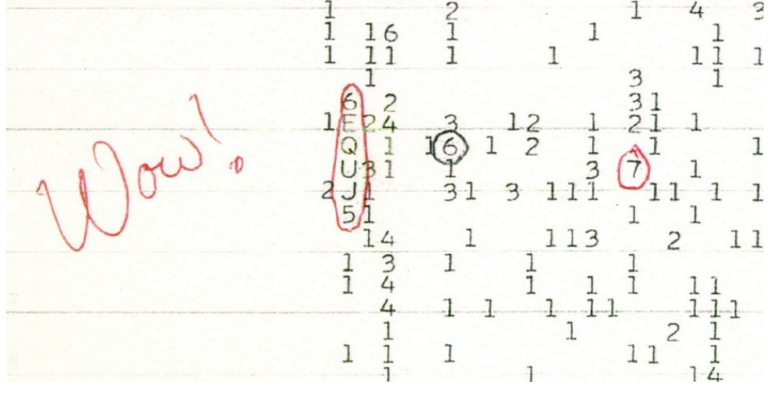
\includegraphics[width=0.5\linewidth]{Figuras/Captura de tela 2025-06-01 094035.png}
\end{figure}

\vspace{0.8cm}

\textcolor{red}{Este é um problema comum na astronomia e para resolvê-lo usarei a distribuição de Poisson, pois a intensidade é uma contagem de fótons, fazendo que essa distribuição seja a mais adequada para o problema. Para verificar se o evento Uau é um sinal aleatório, primeiro vou estimar a média das outras observações, ou seja, o $\lambda$ da distribuição de Poisson.} 

\textcolor{red}{Aqui vou assumir que os espaços vazios são intervalos de 2 segundos onde não houve nenhum fóton, logo sua intensidade será 0, e também vou desconsiderar a coluna do evento Uau nessa estimativa. Considerando 22 colunas e 17 linhas, temos:}

\vspace{0.8cm}

\begin{lstlisting}
    values_no_wow_no_zero = c(rep(1,77), rep(2,8), rep(3,10), rep(4,6), rep(6,2), rep(7,1))
    
    values_no_wow = c(values_no_wow_no_zero, rep(0,17*22-length(values_no_wow_no_zero)))

    lambda = mean(values_no_wow)
\end{lstlisting}

\textcolor{red}{Isso resulta em $\lambda\approx0.444$, ou seja, em média temos $0.444$ de intensidade a cada $2$ segundos. Agora, podemos estimar a probabilidade de ocorrer 6EQUJ5 ou mais do que isso em 12 segundos:}
$$
I_{med} = \frac{6 +14+ 26+ 30+ 19+ 5}{6}\approx16.66
$$
$$
P(x>I_{med}) = \int_{I_{med}}^\infty \frac{e^{-\lambda}\lambda^x}{x!} dx
$$
\textcolor{red}{A partir disso, podemos estimar a probabilidade de que isso seja um evento aleatório, usando:}
$$
P_{aleatorio} = 1-P(x>I_{med})=1.862e-21
$$

\begin{lstlisting}
    wow = c(6, 14, 26, 30, 19, 5)
    prob = ppois(mean(wow), lambda=lambda, lower.tail = F)
\end{lstlisting}

\textcolor{red}{Logo, podemos dizer que a probabilidade de que isso seja um evento aleatório é praticamente nula e que é altamente provável que esse evento seja algum fenômeno físico a ser investigado.}